\documentclass{scrreprt}

\usepackage{aligned-overset}
\usepackage{amsmath}
\usepackage{amsthm}
\usepackage{amssymb}
\usepackage{bm}
\usepackage[shortlabels]{enumitem}
\usepackage{hyperref}
\usepackage[utf8]{inputenc}
\usepackage{multicol}
\usepackage{mathtools}
\usepackage{pdflscape}
\usepackage{physics}
\usepackage{polynom}
\usepackage{tabularx}
\usepackage[table]{xcolor}
\usepackage{titling}
\usepackage{fancyhdr}
\usepackage{xfrac}
\usepackage{pgfplots}

\pgfplotsset{compat = newest}
\usetikzlibrary{arrows, arrows.meta}
\usetikzlibrary{calc}

\author{Karsten Lehmann \\ 4935758}
\date{WiSe 2024/25}
\title{Nachbereitungsaufgaben 5\\INF-B-110, Diskrete Strukturen}

\setlength{\headheight}{26pt}
\pagestyle{fancy}
\fancyhf{}
\lhead{\thetitle}
\rhead{\theauthor}
\lfoot{\thedate}
\rfoot{Seite \thepage}

\newcommand{\ggT}[0]{\text{ggT}}
\DeclarePairedDelimiter{\floor}{\lfloor}{\rfloor}

\begin{document}
\paragraph{N5}
\begin{enumerate}[(a)]
\item Berechnen Sie die Anzahl der Teiler der Zahl 111111.

  \subparagraph{Lsg.} Bestimmen wir zuerst die Primfaktoren der Zahl
  $111111$.
  Mit gängigen Teilbarkeitsregeln fällt schnell auf
  $111111 = 3 \cdot 37037 = 3 \cdot 37 \cdot 1001$.

  Schließlich ist

  $111111 = 3 \cdot 11 \cdot 37 \cdot 91 = 3 \cdot 7 \cdot 11 \cdot 13 \cdot 37$.

  Nun sind alle Teiler von 111111 Produkte dieser 5 Primfaktoren, in denen die
  Primfaktoren entweder nicht oder einmal als Faktor auftauchen können.
  Folglich gibt es $2^5 = 32$ unterschiedliche Produkte dieser Primfaktoren und
  damit hat 111111 auch 32 Teiler.

\item Berechnen Sie mit dem erweiterten euklidischen Algorithmus den
  $\ggT\qty\big(230, 84)$ und stellen Sie ihn in der Form
  $\ggT\qty\big(m, n) = a \cdot n + b \cdot m$ mit
  $a, b \in \mathbb{Z}$ dar.

  \subparagraph{Lsg.} Es soll E-EUKLID$\qty\big(84, 230)$ bestimmt werden

  \begin{tikzpicture}
    \node[anchor=west] at (0,0) {Es ist nicht $84|230$, also berechne E-EUKLID$\qty\big(230 \mod 84, 84)$};
    \node[anchor=west] at (1.5,-.7) {Es ist nicht $62|84$, also berechne E-EUKLID$\qty\big(84 \mod 62, 62)$};
    \node[anchor=west] at (3,-1.4) {Es ist nicht $22|62$, also berechne E-EUKLID$\qty\big(62 \mod 22, 22)$};
    \node[anchor=west] at (4.5,-2.1) {Es ist nicht $18|22$, also berechne E-EUKLID$\qty\big(22 \mod 18, 18)$};
    \node[anchor=west] at (6,-2.8) {Es ist nicht $4|18$, also berechne E-EUKLID$\qty\big(18 \mod 4, 4)$};
    \node[anchor=west] at (7.5,-3.5) {Es ist $2|4$, also gib \hspace{.9cm} zurück};
    \node[anchor=center] (ab5) at (11.3, -3.5) {$\qty\big(1, 0)$};

    \node[anchor=west] at (6, -4.7) {Setze \hspace{2.1cm} und gib \hspace{2.1cm} zurück};
    \node[anchor=west] (res4) at (7, -4.7) {$a' = 1, b' = 0$};
    \node[anchor=center] (ab4) at (11.8, -4.7) {$\qty(0 - 1 \floor{\frac{18}{4}}, 1)$};

    \node[anchor=west] at (4.5, -5.9) {Setze \hspace{2.4cm} und gib \hspace{2.5cm} zurück};
    \node[anchor=west] (res3) at (5.5, -5.9) {$a' = -4, b' = 1$};
    \node[anchor=center] (ab3) at (10.8, -5.9) {$\qty(1 + 4 \floor{\frac{22}{18}}, -4)$};

    \node[anchor=west] at (3, -7.1) {Setze \hspace{2.4cm} und gib \hspace{2.6cm} zurück};
    \node[anchor=west] (res2) at (4, -7.1) {$a' = 5, b' = -4$};
    \node[anchor=center] (ab2) at (9.4, -7.1) {$\qty(-4 - 5 \floor{\frac{62}{22}}, 5)$};

    \node[anchor=west] at (1.5, -8.3) {Setze \hspace{2.6cm} und gib \hspace{2.9cm} zurück};
    \node[anchor=west] (res1) at (2.5, -8.3) {$a' = -14, b' = 5$};
    \node[anchor=center] (ab1) at (8.2, -8.3) {$\qty(5 + 14 \floor{\frac{84}{62}}, -14)$};

    \node[anchor=west] at (0, -9.5) {Setze \hspace{2.8cm} und gib \hspace{3.4cm} zurück};
    \node[anchor=west] (res0) at (1, -9.5) {$a' = 19, b' = -14$};
    \node[anchor=center] (ab0) at (7.2, -9.5) {$\qty(-14 - 19 \floor{\frac{84}{230}}, 19)$};

    \node[anchor=west] at (0, -10.7) {Somit ist \hspace{2.8cm} und $\ggT\qty\big(84, 230) = - 52 \cdot 84 + 19 \cdot 230 = 2$};
    \node[anchor=west] (res) at (1.8, -10.7) {$a = -52, b = 19$};

    \draw[->] (ab5) |- ($(res4)!0.5!(ab5)$) -| (res4);
    \draw[->] (ab4) |- ($(res3)!0.5!(ab4)$) -| (res3);
    \draw[->] (ab3) |- ($(res2)!0.5!(ab3)$) -| (res2);
    \draw[->] (ab2) |- ($(res1)!0.5!(ab2)$) -| (res1);
    \draw[->] (ab1) |- ($(res0)!0.5!(ab1)$) -| (res0);
    \draw[->] (ab0) |- ($(res)!0.5!(ab0)$) -| (res);
  \end{tikzpicture}

\item Berechnen Sie die letzte Ziffer der Zahl $7^{543}$ mit der Methode
  ``Quadrieren und Multiplizieren''.

  \subparagraph{Lsg.} Es ist $\text{bin}\qty\big(543) = 1000011111$.
  Also ist $543 = 2^9 + 2^4 + 2^3 + 2^2 + 2^1 + 2^0$ und folglich
  \[
    7^{543} = 7^{2^9} \cdot 7^{2^4} \cdot 7^{2^3} \cdot 7^{2^2} \cdot 7^{2^1} \cdot 7^{2^0} =
    \qty(\qty(\qty(\qty(\qty(7^{2 \cdot 2 \cdot 2 \cdot 2 \cdot 2} \cdot 7)^2 \cdot 7)^2 \cdot 7)^2 \cdot 7)^2 \cdot 7)
  \]
  Um die letzte Ziffer von $7^{543}$ zu bestimmen, muss $7^{543} \mod 10$
  gerechnet werden.
  Dank der \emph{Homomorphieregel} lässt sich diese Rechnung für jeden
  Zwischenschritt durchführen.
  Die Zwischenergebnisse sind

  \begin{tabular}{|c|c|}
    \hline
    1 & $7 \mod 10 = \colorbox{yellow}{$7$}$ \\
    \hline
    0 & $\colorbox{yellow}{$7$}^2 \mod 10 = \colorbox{blue!20}{$9$}$ \\
    \hline
    0 & $\colorbox{blue!20}{$9$}^2 \mod 10 = \colorbox{orange!20}{$1$}$ \\
    \hline
    0 & $\colorbox{orange!20}{$1$}^2 \mod 10 = \colorbox{green!20}{$1$}$ \\
    \hline
    0 & $\colorbox{green!20}{$1$}^2 \mod 10 = \colorbox{red!20}{$1$}$ \\
    \hline
    1 & $\colorbox{red!20}{$1$}^2 \cdot 7 \mod 10 = \colorbox{teal!20}{$7$}$ \\
    \hline
    1 & $\colorbox{teal!20}{$7$}^2 \cdot 7 \mod 10 = \colorbox{lime!20}{$3$}$ \\
    \hline
    1 & $\colorbox{lime!20}{$3$}^2 \cdot 7 \mod 10 = \colorbox{magenta!20}{$3$}$ \\
    \hline
    1 & $\colorbox{magenta!20}{$3$}^2 \cdot 7 \mod 10 = \colorbox{cyan!20}{$3$}$ \\
    \hline
    1 & $\colorbox{cyan!20}{$3$}^2 \cdot 7 \mod 10 = \colorbox{olive!20}{$3$}$ \\
    \hline
  \end{tabular}

  $\Rightarrow$ die letzte Ziffer von $7^{543}$ ist $\colorbox{olive!20}{$3$}$


\end{enumerate}
\end{document}
